\chapter[Especificação do jogo]{Especificação do jogo}
\addcontentsline{toc}{chapter}{Especificação do jogo}
\markboth{Especificação do jogo}{Especificação do jogo}

Neste capítulo, apresentamos os conceitos gerais do jogo produzido, desde o objetivo, narrativa, regras, mecânicas e funcionalidades. A especificação do jogo é um documento essencial para definir de maneira clara e detalhada todos os aspectos que compõem a experiência do jogador, servindo como guia tanto para a equipe de desenvolvimento quanto para possíveis ajustes e melhorias no decorrer do projeto. A partir desta especificação, é possível alinhar as expectativas e assegurar que o produto final atenda aos requisitos propostos, oferecendo uma base sólida para a implementação e testes do jogo.

\section{Narrativa}

O jogo tem várias inspirações, sendo a principal delas a série “Tron – Uma Odisseia Eletrônica”. Ele utiliza a mecânica dos \textit{light-cycles}, que são rastros deixados pelos jogadores no filme. \textit{Light-cycle} é um sub-jogo da série no qual o objetivo é forçar os jogadores a colidirem com a parede ou com os rastros de luz deixados pelos demais, muito similar ao clássico jogo \textit{Snake}, também conhecido como jogo da cobrinha, mas com elementos de \textit{battle royale}.

Outra inspiração relevante é o jogo de navegador “Curve Fever”, cuja proposta é semelhante à adotada neste projeto. A ideia é criar uma versão renovada do jogo para guiar o aprendizado.

\begin{figure}[htbp]
    \centering
    \caption{Jogo achtung die kurve}
    \label{fig:achtung-kurve}
    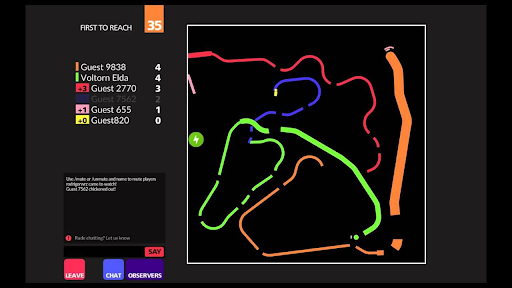
\includegraphics[width=0.7\textwidth]{figuras/kuver-fever.png}
    \legend{Fonte: Thumb video (Let 's Play ACHTUNG DIE KURVE!  Gameplay. Voltorn Elda)}
\end{figure}

A narrativa do jogo é relativamente simples. Até 6 jogadores podem ingressar numa sala virtual, onde cada um controla um dos 6 animais disponíveis. Cada animal é representado por uma cor específica: porco (rosa), dragão (vermelho), serpente (verde), baleia (azul), lobo (branco) e águia (amarelo).

Os jogadores competem em várias rodadas e acumulam pontos de acordo com sua colocação. O número de pontos necessários para o fim da partida é definido pela fórmula:

\begin{center}
    \textbf{Pontuação para vitória = número de jogadores $\times$ 5}
\end{center}

O número mínimo de jogadores para iniciar uma partida é 2. A pontuação obtida em cada rodada segue a regra:

\begin{center}
    \textbf{Pontos da rodada = número de jogadores $-$ colocação do jogador}
\end{center}

O primeiro jogador a atingir a pontuação definida é coroado como \textit{Rei dos Animais}.

\section{Objetivo do Jogo}

O objetivo do jogo é sobreviver o maior tempo possível dentro de um cenário limitado. Por se tratar de um jogo competitivo \textit{PvP}, o último jogador vivo será o vitorioso na rodada.

Para alcançar esse objetivo, os jogadores podem adotar estratégias variadas, utilizar poderes especiais que tornam a partida mais caótica, além de exigir habilidade motora para controlar seu personagem com precisão.

\section{Estrutura da Fase}

A estrutura da fase é simples: uma caixa com tamanho adaptável ao número de jogadores, fundo cinza-escuro e bordas cinza-claro. Ao lado da arena, há um placar exibindo a colocação dos jogadores.

Ao final de cada rodada, a área de jogo é limpa e os jogadores são reposicionados em suas posições iniciais.

\section{Poderes e Habilidades}

O jogo oferece uma habilidade padrão e diversos poderes especiais que surgem aleatoriamente durante a partida.

A habilidade padrão consiste em deixar um rastro letal por onde o personagem se move, capaz de eliminar qualquer jogador (inclusive o próprio). O rastro pode ocasionalmente conter brechas que permitem a passagem.

Os poderes especiais aparecem aleatoriamente no mapa. Ao serem coletados, são ativados imediatamente e têm duração de 7 segundos. Eles podem ajudar ou prejudicar o jogador que os coletou ou afetar os demais.

\begin{itemize}
    \item +Velocidade
    \item -Velocidade
    \item +Velocidade para os outros
    \item -Velocidade para os outros
    \item Inverter controles para os outros
    \item Andar em 90º
    \item Tornar bordas atravessáveis
    \item Limpar mapa
    \item Voar
    \item +Tamanho
    \item -Tamanho
\end{itemize}
\textbf{Poderes verdes:} aplicam-se somente ao jogador que os coletou.\\
\textbf{Poderes vermelhos:} afetam todos os outros jogadores.\\
\textbf{Poderes azuis:} afetam todos os jogadores.

Para uma descrição visual dos poderes, consulte o \textbf{Apêndice 2}.

\section{Mecânicas e Jogabilidade}

A mecânica do jogo é simples: o jogador pode mover-se para a esquerda ou para a direita. No entanto, a movimentação dos personagens é limitada a curvas com raio pré-determinado. A velocidade do jogador influencia diretamente o tamanho da curva: quanto maior a velocidade, maior será o raio da curva.

\section{Gamificação e Análise Crítica}

A escolha desse tipo de jogo envolveu diversos fatores, como a facilidade de criação de \textit{assets} (arte do jogo), o desenvolvimento simples de roteiros e o curto prazo de tempo. O foco principal deste projeto é utilizá-lo como estudo de caso, visando gerar resultados relevantes para a pesquisa.

Apesar da mecânica ser simples, o jogo conta com diversas funcionalidades, como poderes especiais e regras que o tornam dinâmico e interessante.

Além disso, o jogo foi analisado com base no \textit{framework} Octalysis, desenvolvido pelo designer Yu-kai Chou, com o objetivo de avaliar o engajamento dos jogadores. Embora o Octalysis seja um \textit{framework} voltado para a gamificação, ele também pode ser aplicado à análise de jogos, pois oferece uma compreensão profunda das motivações que mantêm os jogadores envolvidos e da efetividade do \textit{game design}.

O Octalysis é composto por oito \textit{cores} (motivações), que são elementos-chave para o engajamento. Na análise, selecionamos os principais \textit{cores} presentes no jogo e os avaliamos em uma escala de 1 a 5, onde 1 indica pouco explorado e 5 indica muito explorado \cite{octalysis}.

\subsection*{Principais \textit{cores} utilizados}

\textbf{Epic Meaning}
\textit{Resumo}: Este \textit{core} refere-se ao senso de propósito maior ou missão.
\textit{Uso}: 2 — Embora a narrativa envolva os animais na floresta, ela não é muito explorada e serve principalmente para criar um ambiente visual, sem grande impacto no engajamento do jogador.

\vspace{0.5em}
\textbf{Social Influence \& Relatedness}
\textit{Resumo}: Relacionado à interação social e senso de comunidade.
\textit{Uso}: 4 — Como o jogo é competitivo, a interação entre os jogadores é um ponto-chave. A disputa aumenta o engajamento e a imersão, estimulando o sentimento de conexão e rivalidade.

\vspace{0.5em}
\textbf{Unpredictability \& Curiosity}
\textit{Resumo}: Este \textit{core} envolve a curiosidade e o desejo de explorar.
\textit{Uso}: 3 — A presença de poderes aleatórios e a variabilidade no comportamento dos jogadores tornam o jogo imprevisível, mantendo o jogador curioso sobre os resultados de cada partida.

\vspace{0.5em}
\textbf{Loss \& Avoidance}
\textit{Resumo}: Refere-se ao medo de perder e à motivação para evitar consequências negativas.
\textit{Uso}: 2 — Embora o jogo seja competitivo, a perda não é tratada como uma consequência punitiva. A penalização ocorre principalmente na pontuação, com perdas menores nas rodadas, o que suaviza o impacto da derrota e foca mais no progresso do jogador.
